Once we have a certain amount of raw data, we need to preprocess this data and create data models for our graph. This turned out to be an evolving process and not a fixed decision. Also, an important question that needs to be answered is: what does an edge represent in our graph? Naturally, when an user opens some post on Reddit, they might start reading the first comment. If it doesn't catch their attention, they read the second top comment. They even might continue reading the reply tree to that comment. The nature of this is that the replies are very often context based. To understand the comment of depth 3, you might need to also have read the comments of depth 2 or 1. For this reason we assume that if an user replies to some comment, they have a connection to all the people in that chain of comments. 

We opted for four different data models. Not all were used along the way.

\subsection{Unique Cartesian Link}
This is probably the most natural way to create an undirected graph from our data. All we do is: all users that commented on a post get linked together in a complete graph with edge weight 1. If there is already an edge between two users, the weight of the edge gets increased by 1. This creates an enormously large graph compared to our other data models. This makes computation on the graph very difficult and slow. Also, it doesn't really represent our idea of a relationship between two users. That's why we opted for other models.

\subsection{Deep Link}
In here, we connect each user to the original poster (OP) and to all users who replied to the user's comment. The edges get a weight depending on the depth of the comment and the achieved upvote score. If there is already an edge between the two users, the weight gets increased. This is a directed graph. See Figure \ref{fig:graphmodel} and the corresponding table.

\begin{table}
\centering
\begin{tabular}{l}
User 0 (OP, depth=1, score=30)  \\
\hline
\hspace{1cm} User 1 (d=1, s=10)              \\
\hline
\hspace{2cm} User 2 (d=2, s=10)            \\
\hline
\hspace{2cm} User 3 (d=2, s=2)             \\
\hline
\hspace{1cm} User 4 (d=1, s=5)             \\
\hline
\hspace{1cm} User 5 (d=1, s=3)             \\
\hline
\hspace{2cm} User 6 (d=2, s=2)             \\
\hline
\hspace{3cm} User 3 (d=3, s=1)             \\
\hline
\hspace{2cm} User  7 (d=2, s=1)            \\
\hspace{6.5cm}
\end{tabular}
\caption{A typical Reddit post, where an indentation represents a reply to the above comment.}
\end{table}

\begin{figure}[H]
    \centering
    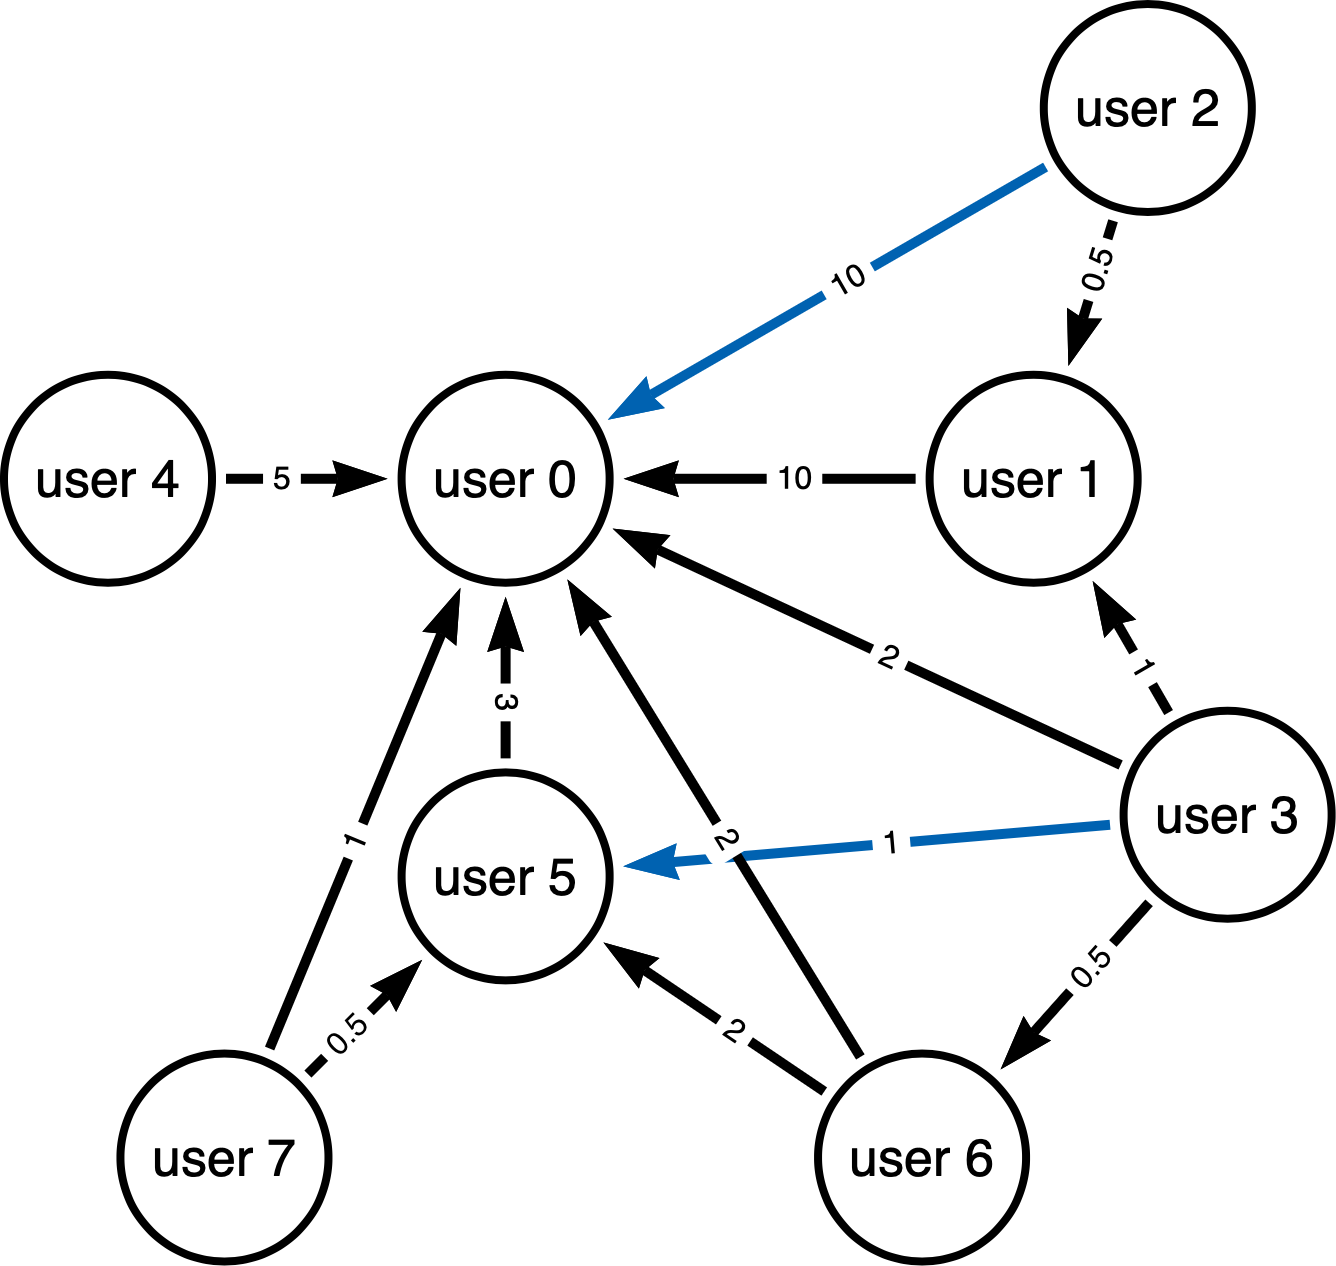
\includegraphics[width=0.3\textwidth]{figures/graph_model.png}
    \caption{The graph representing the above post. The weight is computed as the score of the comment of user$_i$ divided by the depth of the user$_j$, who is above the user$_i$.}
    \label{fig:graphmodel}
\end{figure}


%User 0 (OP, depth=1, score=30)
% 	- User 1 (d=1, s=10)
% 		- User 2 (d=2, s=10)
% 		- User 3 (d=2, s=2)
% 	- User 4 (d=1, s=5)
% 	- User 5 (d=1, s=3)
% 		- User 6 (d=2, s=2)
% 			- User 3 (d=3, s=1)
% 		-User  7 (d=2, s=1)

% figure graph_model


\subsection{Next Link}
Same as Deep Link, except that we only connect each user to the OP and the immediate users who commented directly on the user's comment. Thus the blue link in Figure \ref{fig:graphmodel} are missing in this data model. Also a directed graph.

\subsection{Deep Link No Merge}
The same as Deep Link but here we don't merge the weights and allow multiple edges from one user to another. Thus, this is a directed multigraph. We found that this approach has still lots of information but is not too expensive to compute.











